% laboratory measurements
\subsection{Laborversuche}


\begin{frame}
\frametitle{Triaxialversuch}

\begin{figure}
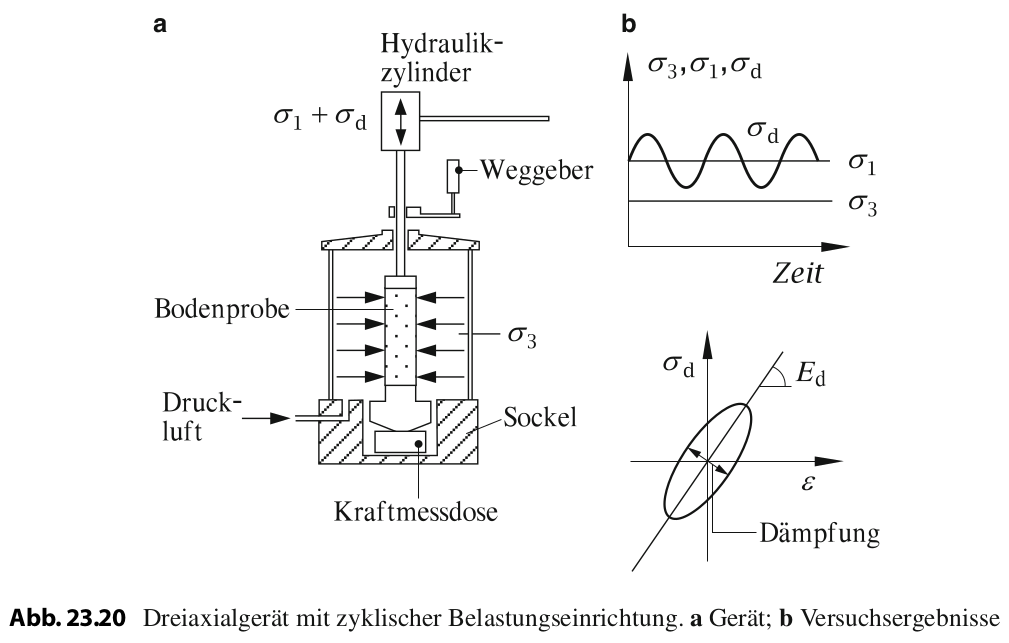
\includegraphics[width=0.82\textwidth]{fig_img/triaxial_test.png}
\cite{Schmidt2017}
\end{figure}
%anisotrope Spannungszustände 
% Einfluss der Belastungsamplitude, Zyklenzahl
% große Verformungen, kleine Frequenzen
\end{frame}


\begin{frame}
\frametitle{Schwingversuche}

\begin{figure}
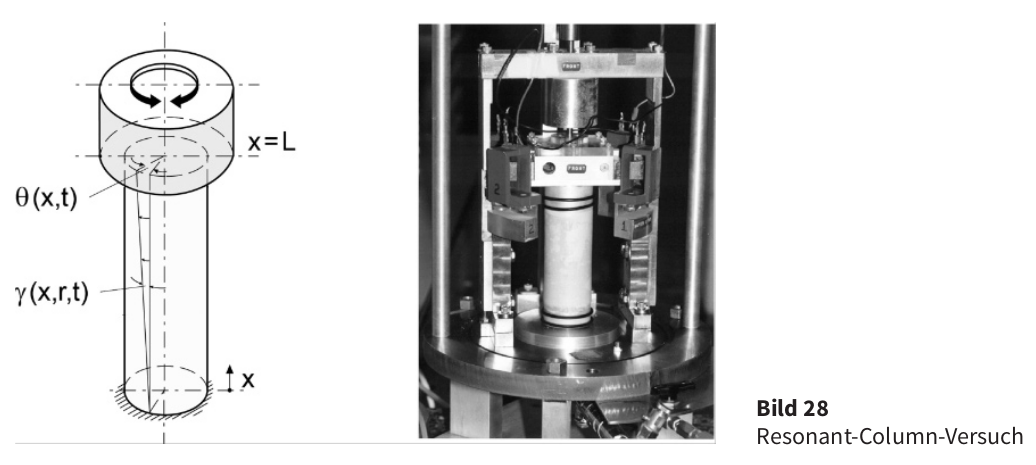
\includegraphics[width=0.91\textwidth]{fig_img/resonant_column.png}
\cite{Vrettos2017}
\end{figure}

Eigenfrequenz $\leadsto$ Schubmodul, Frequenzgang oder Ausschwingen $\leadsto$ Dämpfung, \textsl{siehe Übung}.
\end{frame}


\begin{frame}
\frametitle{Weitere Verfahren}
\begin{itemize}
 \item Scherversuche 

        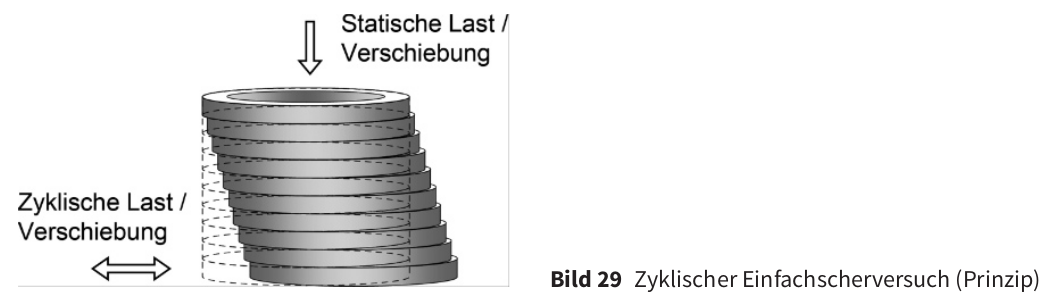
\includegraphics[width=0.84\textwidth]{fig_img/shear_test.png} \cite{Vrettos2017}
 
 \item Ultraschallmessung, ähnlich zu Bohrlochmessungen im Gelände
\end{itemize}



\end{frame}
